%  LaTeX support: latex@mdpi.com 
%  For support, please attach all files needed for compiling as well as the log file, and specify your operating system, LaTeX version, and LaTeX editor.

%=================================================================
\documentclass[journal,article,submit,pdftex,moreauthors]{Definitions/mdpi} 

%--------------------
% Class Options:
%--------------------
%----------
% journal
%----------
% Choose between the following MDPI journals:
% acoustics, actuators, addictions, admsci, adolescents, aerobiology, aerospace, agriculture, agriengineering, agrochemicals, agronomy, ai, air, algorithms, allergies, alloys, analytica, analytics, anatomia, animals, antibiotics, antibodies, antioxidants, applbiosci, appliedchem, appliedmath, applmech, applmicrobiol, applnano, applsci, aquacj, architecture, arm, arthropoda, arts, asc, asi, astronomy, atmosphere, atoms, audiolres, automation, axioms, bacteria, batteries, bdcc, behavsci, beverages, biochem, bioengineering, biologics, biology, biomass, biomechanics, biomed, biomedicines, biomedinformatics, biomimetics, biomolecules, biophysica, biosensors, biotech, birds, bloods, blsf, brainsci, breath, buildings, businesses, cancers, carbon, cardiogenetics, catalysts, cells, ceramics, challenges, chemengineering, chemistry, chemosensors, chemproc, children, chips, cimb, civileng, cleantechnol, climate, clinpract, clockssleep, cmd, coasts, coatings, colloids, colorants, commodities, compounds, computation, computers, condensedmatter, conservation, constrmater, cosmetics, covid, crops, cryptography, crystals, csmf, ctn, curroncol, cyber, dairy, data, ddc, dentistry, dermato, dermatopathology, designs, devices, diabetology, diagnostics, dietetics, digital, disabilities, diseases, diversity, dna, drones, dynamics, earth, ebj, ecologies, econometrics, economies, education, ejihpe, electricity, electrochem, electronicmat, electronics, encyclopedia, endocrines, energies, eng, engproc, entomology, entropy, environments, environsciproc, epidemiologia, epigenomes, est, fermentation, fibers, fintech, fire, fishes, fluids, foods, forecasting, forensicsci, forests, foundations, fractalfract, fuels, future, futureinternet, futurepharmacol, futurephys, futuretransp, galaxies, games, gases, gastroent, gastrointestdisord, gels, genealogy, genes, geographies, geohazards, geomatics, geosciences, geotechnics, geriatrics, grasses, gucdd, hazardousmatters, healthcare, hearts, hemato, hematolrep, heritage, higheredu, highthroughput, histories, horticulturae, hospitals, humanities, humans, hydrobiology, hydrogen, hydrology, hygiene, idr, ijerph, ijfs, ijgi, ijms, ijns, ijpb, ijtm, ijtpp, ime, immuno, informatics, information, infrastructures, inorganics, insects, instruments, inventions, iot, j, jal, jcdd, jcm, jcp, jcs, jcto, jdb, jeta, jfb, jfmk, jimaging, jintelligence, jlpea, jmmp, jmp, jmse, jne, jnt, jof, joitmc, jor, journalmedia, jox, jpm, jrfm, jsan, jtaer, jvd, jzbg, kidneydial, kinasesphosphatases, knowledge, land, languages, laws, life, liquids, literature, livers, logics, logistics, lubricants, lymphatics, machines, macromol, magnetism, magnetochemistry, make, marinedrugs, materials, materproc, mathematics, mca, measurements, medicina, medicines, medsci, membranes, merits, metabolites, metals, meteorology, methane, metrology, micro, microarrays, microbiolres, micromachines, microorganisms, microplastics, minerals, mining, modelling, molbank, molecules, mps, msf, mti, muscles, nanoenergyadv, nanomanufacturing,\gdef\@continuouspages{yes}} nanomaterials, ncrna, ndt, network, neuroglia, neurolint, neurosci, nitrogen, notspecified, %%nri, nursrep, nutraceuticals, nutrients, obesities, oceans, ohbm, onco, %oncopathology, optics, oral, organics, organoids, osteology, oxygen, parasites, parasitologia, particles, pathogens, pathophysiology, pediatrrep, pharmaceuticals, pharmaceutics, pharmacoepidemiology,\gdef\@ISSN{2813-0618}\gdef\@continuous pharmacy, philosophies, photochem, photonics, phycology, physchem, physics, physiologia, plants, plasma, platforms, pollutants, polymers, polysaccharides, poultry, powders, preprints, proceedings, processes, prosthesis, proteomes, psf, psych, psychiatryint, psychoactives, publications, quantumrep, quaternary, qubs, radiation, reactions, receptors, recycling, regeneration, religions, remotesensing, reports, reprodmed, resources, rheumato, risks, robotics, ruminants, safety, sci, scipharm, sclerosis, seeds, sensors, separations, sexes, signals, sinusitis, skins, smartcities, sna, societies, socsci, software, soilsystems, solar, solids, spectroscj, sports, standards, stats, std, stresses, surfaces, surgeries, suschem, sustainability, symmetry, synbio, systems, targets, taxonomy, technologies, telecom, test, textiles, thalassrep, thermo, tomography, tourismhosp, toxics, toxins, transplantology, transportation, traumacare, traumas, tropicalmed, universe, urbansci, uro, vaccines, vehicles, venereology, vetsci, vibration, virtualworlds, viruses, vision, waste, water, wem, wevj, wind, women, world, youth, zoonoticdis 
% For posting an early version of this manuscript as a preprint, you may use "preprints" as the journal. Changing "submit" to "accept" before posting will remove line numbers.

%---------
% article
%---------
% The default type of manuscript is "article", but can be replaced by: 
% abstract, addendum, article, book, bookreview, briefreport, casereport, comment, commentary, communication, conferenceproceedings, correction, conferencereport, entry, expressionofconcern, extendedabstract, datadescriptor, editorial, essay, erratum, hypothesis, interestingimage, obituary, opinion, projectreport, reply, retraction, review, perspective, protocol, shortnote, studyprotocol, systematicreview, supfile, technicalnote, viewpoint, guidelines, registeredreport, tutorial
% supfile = supplementary materials

%----------
% submit
%----------
% The class option "submit" will be changed to "accept" by the Editorial Office when the paper is accepted. This will only make changes to the frontpage (e.g., the logo of the journal will get visible), the headings, and the copyright information. Also, line numbering will be removed. Journal info and pagination for accepted papers will also be assigned by the Editorial Office.

%------------------
% moreauthors
%------------------
% If there is only one author the class option oneauthor should be used. Otherwise use the class option moreauthors.

%---------
% pdftex
%---------
% The option pdftex is for use with pdfLaTeX. Remove "pdftex" for (1) compiling with LaTeX & dvi2pdf (if eps figures are used) or for (2) compiling with XeLaTeX.

%=================================================================
% MDPI internal commands - do not modify
\firstpage{1} 
\makeatletter 
\setcounter{page}{\@firstpage} 
\makeatother
\pubvolume{1}
\issuenum{1}
\articlenumber{0}
\pubyear{2024}
\copyrightyear{2024}
%\externaleditor{Academic Editor: Firstname Lastname}
\datereceived{ } 
\daterevised{ } % Comment out if no revised date
\dateaccepted{ } 
\datepublished{ } 
%\datecorrected{} % For corrected papers: "Corrected: XXX" date in the original paper.
%\dateretracted{} % For corrected papers: "Retracted: XXX" date in the original paper.
\hreflink{https://doi.org/} % If needed use \linebreak
%\doinum{}
%\pdfoutput=1 % Uncommented for upload to arXiv.org
%\CorrStatement{yes}  % For updates


%=================================================================
% Add packages and commands here. The following packages are loaded in our class file: fontenc, inputenc, calc, indentfirst, fancyhdr, graphicx, epstopdf, lastpage, ifthen, float, amsmath, amssymb, lineno, setspace, enumitem, mathpazo, booktabs, titlesec, etoolbox, tabto, xcolor, colortbl, soul, multirow, microtype, tikz, totcount, changepage, attrib, upgreek, array, tabularx, pbox, ragged2e, tocloft, marginnote, marginfix, enotez, amsthm, natbib, hyperref, cleveref, scrextend, url, geometry, newfloat, caption, draftwatermark, seqsplit
% cleveref: load \crefname definitions after \begin{document}

%=================================================================
% Please use the following mathematics environments: Theorem, Lemma, Corollary, Proposition, Characterization, Property, Problem, Example, ExamplesandDefinitions, Hypothesis, Remark, Definition, Notation, Assumption
%% For proofs, please use the proof environment (the amsthm package is loaded by the MDPI class).

%=================================================================


% Full title of the paper (Capitalized)
\Title{Optimalisasi Pencarian Karir dengan JobFit: Menerapkan Teknologi Machine Learning untuk Pencocokan Pekerjaan yang Tepat}

% MDPI internal command: Title for citation in the left column
\TitleCitation{JobFit: Optimalisasi Pencocokan Pekerjaan dengan Machine Learning}

% Author Orchid ID: enter ID or remove command
\newcommand{\orcidauthorA}{0000-0000-0000-000X} % Add \orcidA{} behind the author's name
%\newcommand{\orcidauthorB}{0000-0000-0000-000X} % Add \orcidB{} behind the author's name

% Authors, for the paper (add full first names)
\Author{Muhammad Ardiansyah Asrifah $^{1}$, Jonathan Kwan $^{2}$, Andi Ahmad Fail Fudhayl $^{3}$, Andi Ahmad Salwan $^{4}$, Khalizatul Jannah $^{5}$, Andi Muthia Mulia Putri $^{6}$, Adrian Hidayat $^{7}$}

%\longauthorlist{yes}

% MDPI internal command: Authors, for metadata in PDF
\AuthorNames{Muhammad Ardiansyah Asrifah, Jonathan Kwan, Andi Ahmad Fail Fudhayl, Andi Ahmad Salwan, Khalizatul Jannah, Andi Muthia Mulia Putri, Adrian Hidayat}

% MDPI internal command: Authors, for citation in the left column
\AuthorCitation{Asrifah; Kwan; Fudhayl; Salwan; Jannah; Putri; Hidayat}
% If this is a Chicago style journal: Lastname, Firstname, Firstname Lastname, and Firstname Lastname.

% Affiliations / Addresses (Add [1] after \address if there is only one affiliation.)
\address{%
$^{1}$ \quad Universitas Hasanuddin; asrifahma22h@student.unhas.ac.id\\
$^{2}$ \quad Universitas Hasanuddin; kwanj22h@student.unhas.ac.id\\
$^{3}$ \quad Universitas Hasanuddin; fudhaylaaf22h@student.unhas.ac.id\\
$^{4}$ \quad Universitas Hasanuddin; faridaas22h@student.unhas.ac.id\\
$^{5}$ \quad Universitas Hasanuddin; jannahk22h@student.unhas.ac.id\\
$^{6}$ \quad Universitas Hasanuddin; putriamm22h@student.unhas.ac.id\\
$^{7}$ \quad Universitas Hasanuddin; hidayata22h@student.unhas.ac.id}

% Contact information of the corresponding author
\corres{Correspondence: asrifahma22h@student.unhas.ac.id; Tel.: 086253672134}

% Current address and/or shared authorship
\firstnote{Current address: Jalan Perintis Kemerdekaan Km. 10 Tamalanrea,. Kota: Makassar.}  % Current address should not be the same as any items in the Affiliation section.
\secondnote{These authors contributed equally to this work.}
% The commands \thirdnote{} till \eighthnote{} are available for further notes

%\simplesumm{} % Simple summary

%\conference{} % An extended version of a conference paper

% Abstract (Do not insert blank lines, i.e. \\) 
\abstract{Aplikasi \textit{JobFit} berbasis Android yang menerapkan \textit{machine learning} dirancang untuk mencocokkan keterampilan pengguna dengan kebutuhan perusahaan secara efektif. Dalam penelitian ini, dijelaskan pengembangan aplikasi yang menggunakan algoritma \textit{machine learning} untuk menganalisis profil keterampilan pengguna dan persyaratan pekerjaan. Data keterampilan dikumpulkan melalui kuis interaktif, dan informasi lowongan diambil dari \textit{database}. Aplikasi ini dilatih untuk mengenali pola kecocokan antara kedua \textit{dataset} tersebut. Hasil awal menunjukkan tingkat akurasi yang tinggi dalam memberikan rekomendasi pekerjaan yang relevan, serta saran untuk meningkatkan kompetensi pengguna. Dengan demikian, aplikasi ini tidak hanya memudahkan pencari kerja dalam menemukan posisi yang sesuai, tetapi juga membantu perusahaan dalam menemukan kandidat yang tepat, sehingga meningkatkan efisiensi dalam proses rekrutmen dan pencarian kerja.}

% Keywords
\keyword{Machine Learning; Pegawai; Perusahaan} 

% The fields PACS, MSC, and JEL may be left empty or commented out if not applicable
%\PACS{J0101}
%\MSC{}
%\JEL{}

%%%%%%%%%%%%%%%%%%%%%%%%%%%%%%%%%%%%%%%%%%
% Only for the journal Diversity
%\LSID{\url{http://}}

%%%%%%%%%%%%%%%%%%%%%%%%%%%%%%%%%%%%%%%%%%
% Only for the journal Applied Sciences
%\featuredapplication{Authors are encouraged to provide a concise description of the specific application or a potential application of the work. This section is not mandatory.}
%%%%%%%%%%%%%%%%%%%%%%%%%%%%%%%%%%%%%%%%%%

%%%%%%%%%%%%%%%%%%%%%%%%%%%%%%%%%%%%%%%%%%
% Only for the journal Data
%\dataset{DOI number or link to the deposited data set if the data set is published separately. If the data set shall be published as a supplement to this paper, this field will be filled by the journal editors. In this case, please submit the data set as a supplement.}
%\datasetlicense{License under which the data set is made available (CC0, CC-BY, CC-BY-SA, CC-BY-NC, etc.)}

%%%%%%%%%%%%%%%%%%%%%%%%%%%%%%%%%%%%%%%%%%
% Only for the journal Toxins
%\keycontribution{The breakthroughs or highlights of the manuscript. Authors can write one or two sentences to describe the most important part of the paper.}

%%%%%%%%%%%%%%%%%%%%%%%%%%%%%%%%%%%%%%%%%%
% Only for the journal Encyclopedia
%\encyclopediadef{For entry manuscripts only: please provide a brief overview of the entry title instead of an abstract.}

%%%%%%%%%%%%%%%%%%%%%%%%%%%%%%%%%%%%%%%%%%
% Only for the journal Advances in Respiratory Medicine and Smart Cities
%\addhighlights{yes}
%\renewcommand{\addhighlights}{%

%\noindent This is an obligatory section in “Advances in Respiratory Medicine'' and ``Smart Cities”, whose goal is to increase the discoverability and readability of the article via search engines and other scholars. Highlights should not be a copy of the abstract, but a simple text allowing the reader to quickly and simplified find out what the article is about and what can be cited from it. Each of these parts should be devoted up to 2~bullet points.\vspace{3pt}\\
%\textbf{What are the main findings?}
% \begin{itemize}[labelsep=2.5mm,topsep=-3pt]
% \item First bullet.
% \item Second bullet.
% \end{itemize}\vspace{3pt}
%\textbf{What is the implication of the main finding?}
% \begin{itemize}[labelsep=2.5mm,topsep=-3pt]
% \item First bullet.
% \item Second bullet.
% \end{itemize}
%}

%%%%%%%%%%%%%%%%%%%%%%%%%%%%%%%%%%%%%%%%%%
\begin{document}

%%%%%%%%%%%%%%%%%%%%%%%%%%%%%%%%%%%%%%%%%%
\setcounter{section}{-1} %% Remove this when starting to work on the template.

% The order of the section titles is different for some journals. Please refer to the "Instructions for Authors” on the journal homepage.

\section{Introduction}

\subsection{Project Charter}

\subsubsection{Tahapan Perencanaan}

\begin{table}[ht]
\centering
\begin{tabular}{|c|c|}
\hline
\textbf{Nama} & \textbf{Role} \\
\hline
Muhammad Ardiansyah Asrifah & Project Manager \\
Khalizatul Jannah & Ilustrator \\
Andi Ahmad Fa'il Fudhayl & UI/UX Engineer \\
Jonathan Kwan & Quality Assurance \\
Andi Ahmad Salwan & Programmer \\
Andi Muthia Mulia Putri & AI Engineer \\
Adrian Hidayat & Programmer \\
\hline
\end{tabular}
\captionsetup{justification=centering}
\caption{Pembagian \textit{Role} Tim}
\end{table}

\subsubsection{Project Description}
Proyek ini merupakan inisiatif untuk dibuatnya aplikasi berbasis kecerdasan buatan (\textit{AI}) bernama \textit{Jobfit}, yang dirancang khusus untuk mengoptimalkan proses rekrutmen. Dengan \textit{Jobfit}, kemudahan dan kecepatan dalam pencocokan kualifikasi pelamar dengan kebutuhan perusahaan dapat dirasakan oleh perusahaan maupun pelamar kerja secara lebih akurat. Berbagai proses dalam rekrutmen, seperti penyaringan CV dan pencocokan antara kualifikasi kandidat dengan persyaratan posisi yang ditawarkan, diotomatisasi melalui aplikasi ini. Algoritma berbasis \textit{machine learning} diterapkan dalam \textit{Jobfit} untuk memproses data pelamar secara efisien dan akurat, sehingga proses rekrutmen dapat dipercepat, efisiensi biaya dapat ditingkatkan, dan potensi bias dapat dikurangi.

Di era persaingan ketat dan perkembangan teknologi yang pesat ini, optimalisasi proses rekrutmen melalui \textit{AI} dipilih sebagai strategi untuk memastikan bahwa setiap kandidat yang direkrut benar-benar sesuai dengan kebutuhan perusahaan atau instansi. Dengan adanya \textit{Jobfit}, pengalaman rekrutmen yang lebih baik, lebih transparan, dan bebas dari bias dapat diperoleh oleh perusahaan dan pelamar.

\subsubsection{SMART Question}
Aplikasi pencocokan calon pegawai ini dirancang untuk meningkatkan efisiensi proses rekrutmen di instansi atau perusahaan dengan memanfaatkan teknologi \textit{machine learning} untuk menyaring dan mencocokkan kandidat secara otomatis berdasarkan keterampilan dan kualifikasi yang dibutuhkan. Dengan aplikasi ini, proses seleksi diharapkan dapat dilakukan dengan lebih cepat dan akurat, sehingga waktu yang dibutuhkan untuk menilai setiap kandidat secara manual dapat dikurangi. Dalam 6 bulan pertama setelah implementasi, peningkatan signifikan dalam kecepatan proses seleksi kandidat diharapkan terjadi dibandingkan dengan metode manual yang sebelumnya diterapkan. Secara spesifik, tujuan dari aplikasi ini adalah untuk meningkatkan efisiensi proses seleksi dengan mengurangi waktu yang dihabiskan untuk mencari dan mengevaluasi kandidat yang sesuai.

Target realistis juga telah ditetapkan oleh tim pengembang untuk mencapai \textit{milestone} proyek, termasuk pengujian \textit{beta}, dalam waktu 16 pekan. Diharapkan bahwa pengujian \textit{beta} ini dapat memberikan umpan balik yang berharga untuk perbaikan dan penyempurnaan aplikasi sebelum dirilis dalam versi final. Inisiatif perusahaan dalam meningkatkan transparansi dan akuntabilitas dalam proses rekrutmen juga didukung oleh aplikasi ini, dengan meminimalkan potensi bias dan memastikan bahwa semua kandidat dievaluasi berdasarkan data dan kualifikasi yang objektif. Dengan menggunakan teknologi ini, diharapkan proses rekrutmen dapat dilakukan secara adil dan efisien. Pada akhirnya, aplikasi ini diharapkan dapat dirilis dalam versi \textit{beta} yang fungsional dalam waktu 16 pekan, memberikan solusi praktis untuk mengoptimalkan alur rekrutmen di perusahaan.

\subsubsection{Alat / Tools}
\begin{enumerate}[left=2em]
    \item Android Studio
    \item Figma
    \item Google Collab
    \item Ibis Paint
\end{enumerate}

\subsubsection{Target User}
\begin{enumerate}[left=2em]
    \item Masyarakat Umum
    \item Pekerja
    \item Perusahaan
\end{enumerate}

\subsection{Situasi dan Kondisi Sekarang}

Saat ini, proses rekrutmen di Indonesia masih dilakukan dengan metode yang relatif konvensional, meskipun sistem online untuk pendaftaran seperti SSCASN (Sistem Seleksi Calon Aparatur Sipil Negara) sudah tersedia. Proses ini biasanya melibatkan beberapa tahapan seperti seleksi administrasi, ujian kompetensi dasar (SKD), dan ujian kompetensi bidang (SKB), yang sering kali memakan waktu yang panjang dan sumber daya yang besar. Selain itu, penilaian kandidat masih sangat bergantung pada sistem manual yang membuka peluang terjadinya bias dan ketidakefisienan.

Beberapa tantangan yang sering dihadapi adalah:
\begin{itemize}[left=2em]
    \item \textbf{Beban administratif yang berat:} Jumlah pelamar yang besar menyebabkan waktu dan tenaga panitia seleksi harus dihabiskan untuk menyaring data dan dokumen secara manual.
    \item \textbf{Keterbatasan dalam pencocokan posisi:} Meskipun proses seleksi ujian objektif, tahap selanjutnya dalam pencocokan kandidat dengan posisi yang tepat masih sering tidak optimal karena keterbatasan sumber daya untuk analisis mendalam.
    \item \textbf{Kurangnya transparansi dan akurasi:} Sistem manual memiliki potensi terjadinya ketidakakuratan atau bias yang dapat mempengaruhi hasil seleksi.
\end{itemize}

\subsection{Proyek Sebelumnya yang Mirip}

Proyek \textit{Jobfit} yang berbasis AI memang belum banyak dikembangkan secara khusus di Indonesia. Namun, di tingkat global, beberapa sistem rekrutmen berbasis AI sudah mulai diterapkan, seperti sistem \textit{Applicant Tracking Systems} (ATS) yang digunakan oleh perusahaan besar untuk menyaring kandidat secara otomatis berdasarkan kata kunci tertentu di dalam CV dan surat lamaran. Sistem ini juga memanfaatkan \textit{Natural Language Processing} (NLP) untuk membantu dalam memahami konteks dari dokumen lamaran secara otomatis. Namun, dalam proses rekrutmen, solusi spesifik berbasis AI yang mencakup proses screening hingga pencocokan posisi yang terintegrasi secara komprehensif dengan sistem pemerintah belum ada. Sebagian besar proyek yang ada di Indonesia masih difokuskan pada peningkatan infrastruktur digital atau pada ujian berbasis komputer seperti \textit{Computer Assisted Test} (CAT). Oleh karena itu, \textit{Jobfit} dianggap sebagai inovasi yang signifikan karena tidak hanya proses penyaringan yang diotomatisasi, tetapi juga rekomendasi yang lebih akurat dan objektif dalam pencocokan kandidat dengan posisi yang tepat dapat diberikan.

\section{Objektif Proyek}

\subsection{Tujuan Proyek}
Proyek \textit{Jobfit} memiliki beberapa tujuan utama dalam mengoptimalkan proses rekrutmen dengan memanfaatkan kecerdasan buatan (\textit{AI}). Adapun tujuan-tujuan dari proyek ini adalah sebagai berikut:
\begin{itemize}[left=2em]
    \item \textbf{Efisiensi Proses Rekrutmen yang Meningkat:} Beban administratif akan dikurangi dengan otomatisasi penyaringan awal dan pencocokan kandidat dengan posisi yang tersedia secara lebih cepat dan efisien.
    \item \textbf{Bias dalam Seleksi yang Dikurangi:} Sistem yang lebih transparan dan objektif akan dihadirkan dalam menyeleksi kandidat berdasarkan kompetensi, pendidikan, dan hasil tes, tanpa dipengaruhi oleh bias manusia yang sering kali bersifat subjektif.
    \item \textbf{Akurasi Pencocokan Kandidat dengan Posisi yang Meningkat:} Kandidat akan dicocokkan secara lebih tepat dengan posisi yang dibuka berdasarkan keahlian, pengalaman, pendidikan, dan hasil tes, dengan menggunakan algoritma \textit{machine learning} yang terus disempurnakan.
    \item \textbf{Alokasi Sumber Daya yang Dioptimalkan:} Waktu dan energi yang digunakan oleh panitia seleksi untuk tugas-tugas administratif akan dikurangi, sehingga mereka dapat lebih fokus pada kandidat yang paling potensial di tahap akhir proses seleksi.
    \item \textbf{Keamanan dan Skalabilitas Data yang Terjamin:} Sistem yang aman sesuai dengan standar keamanan data pemerintah akan diimplementasikan, dengan kemampuan untuk menangani data pelamar dalam jumlah besar dan memastikan infrastruktur sistem dapat diakses secara luas dan mudah.
\end{itemize}

\subsection{Cara Mencapai Tujuan}
Untuk tujuan tersebut, beberapa strategi dan metode akan diterapkan dalam pengembangan serta implementasi aplikasi \textit{Jobfit}:
\begin{itemize}[left=2em]
    \item \textbf{Penerapan Kecerdasan Buatan (\textit{AI}) pada Proses Seleksi:} Teknologi \textit{AI} akan digunakan dalam aplikasi \textit{Jobfit}, yang mencakup:
    \begin{itemize}[left=2em]
        \item \textit{Natural Language Processing (\textit{NLP}):} CV dan surat lamaran pelamar akan dibaca dan dianalisis secara otomatis.
        \item \textit{Machine Learning (\textit{ML}):} Data historis rekrutmen sebelumnya akan dipelajari untuk memprediksi kesesuaian kandidat dengan posisi tertentu.
        \item \textit{Automated Scoring:} Hasil ujian pelamar akan dinilai secara otomatis dan skor prioritas akan diberikan pada kandidat terbaik.
    \end{itemize}
    \item \textbf{Penyaringan dan Pencocokan Otomatis Berdasarkan Kriteria Spesifik:} Kandidat akan disaring secara otomatis berdasarkan kualifikasi yang ditetapkan, seperti tingkat pendidikan, pengalaman kerja, dan kompetensi khusus yang dibutuhkan oleh posisi tertentu.
    \item \textbf{Pengembangan Antarmuka Pengguna yang Ramah:} Antarmuka yang mudah digunakan akan disediakan, baik untuk pelamar, panitia seleksi, maupun HRD pemerintah. Dashboard yang intuitif akan disediakan agar pelamar dapat memantau status lamaran mereka, dan panitia seleksi dapat melakukan pemantauan serta pengelolaan data pelamar dengan mudah.
    \item \textbf{Keamanan Data dan Skalabilitas Infrastruktur:} Enkripsi data akan diimplementasikan untuk menjaga keamanan informasi pelamar. Sistem akan di-host pada infrastruktur berbasis \textit{cloud} yang mampu menangani jutaan data pelamar dan memungkinkan pemrosesan secara real-time.
\end{itemize}

\subsection{Indikator Keberhasilan}
Indikator keberhasilan proyek \textit{Jobfit} dapat diukur melalui beberapa aspek, antara lain:
\begin{itemize}[left=2em]
    \item \textbf{Waktu Penyaringan Awal yang Lebih Cepat:} Keberhasilan aplikasi akan diukur dengan kemampuan untuk menyaring dan mencocokkan data pelamar lebih cepat dibandingkan dengan metode manual. Target yang ditetapkan adalah pengurangan waktu proses seleksi awal hingga 50\%.
    \item \textbf{Penurunan Tingkat Bias dalam Seleksi:} Bias dalam proses seleksi akan dikurangi, yang dapat diukur dari kepuasan pengguna (panitia seleksi dan pelamar) terkait transparansi dan objektivitas hasil seleksi. Hal ini akan dilakukan melalui survei umpan balik setelah pelaksanaan seleksi.
    \item \textbf{Akurasi Pencocokan Kandidat dengan Posisi:} Keberhasilan pencocokan posisi yang lebih akurat dapat diukur dari persentase kandidat yang berhasil lolos hingga tahap akhir seleksi berdasarkan hasil algoritma pencocokan \textit{AI}. Semakin tinggi kesesuaian antara kandidat yang direkomendasikan oleh sistem dengan yang dipilih pada tahap akhir, semakin sukses sistem ini.
    \item \textbf{Jumlah Pelamar yang Diproses secara Efisien:} Sistem harus mampu memproses jutaan data pelamar setiap tahunnya dengan lancar dan tanpa gangguan, dengan target keberhasilan dalam menangani minimal 95\% dari total pelamar secara efisien.
    \item \textbf{Pengurangan Beban Administratif Panitia Seleksi:} Indikator lain adalah pengurangan beban administrasi yang akan diukur melalui penurunan jumlah waktu yang dihabiskan oleh panitia seleksi pada tugas administratif.
\end{itemize}

\section{Materials and Methods}
\subsection{Data Collection}
Pengumpulan data untuk aplikasi ini dilakukan dengan mengambil dataset dari Kaggle, salah satu platform terbesar yang menyediakan berbagai dataset untuk penelitian, pengembangan, dan proyek analisis data. Kaggle memiliki beragam dataset dari berbagai kategori, mulai dari kesehatan, finansial, hingga pekerjaan dan rekrutmen. Kami memilih dataset yang relevan dengan topik aplikasi ini, yaitu pencocokan kandidat pekerjaan atau analisis rekrutmen.

\begin{figure}[H]
    \centering
    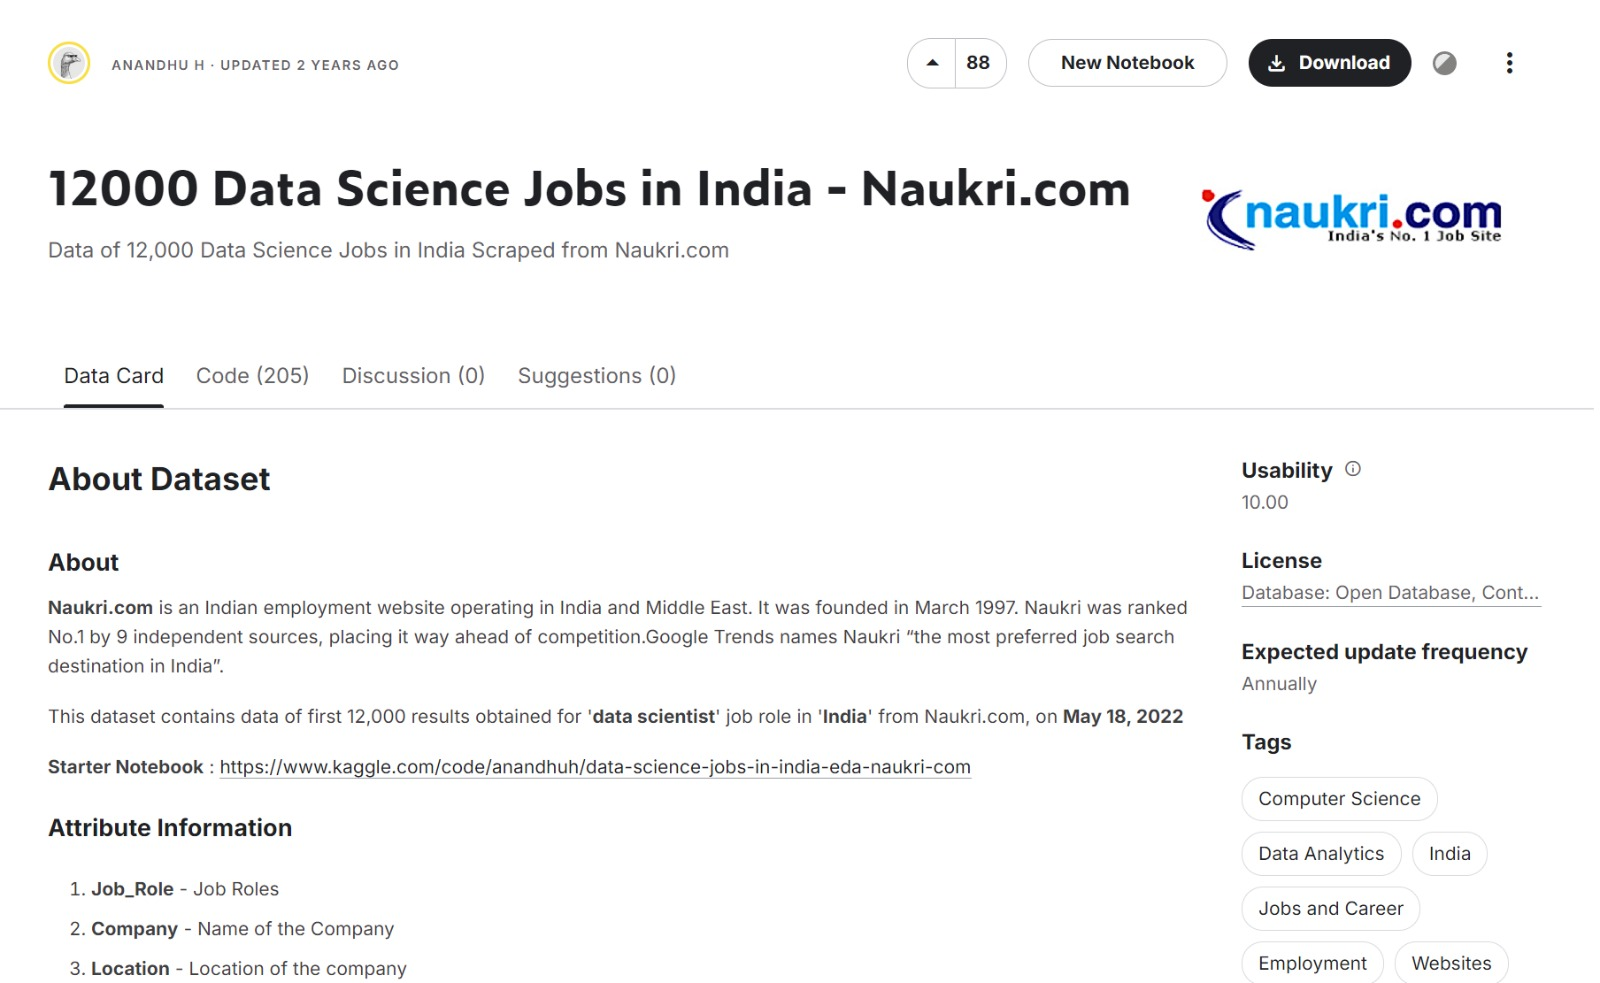
\includegraphics[width=0.8\textwidth]{image/datasetkaggle.jpeg} % 
    \captionsetup{justification=centering}
    \caption{Halaman \textit{Dataset} di \textit{Kaggle}}
    \label{fig:kaggle}
\end{figure}

\subsection{Data Explanation}
\textit{Dataset} yang digunakan dalam aplikasi pencocokan calon pegawai ini diambil dari \textit{Kaggle}, sebuah platform yang menyediakan berbagai kumpulan data untuk analisis dan pengembangan model \textit{machine learning}. \textit{Dataset} yang dipilih untuk proyek ini difokuskan pada informasi mengenai kandidat pekerjaan dan pekerjaan yang tersedia, yang mencakup berbagai atribut penting seperti keterampilan, pengalaman, pendidikan, dan lokasi geografis. Data ini digunakan sebagai dasar untuk menganalisis kesesuaian antara kandidat dan pekerjaan yang mereka minati.

\begin{figure}[H]
    \centering
    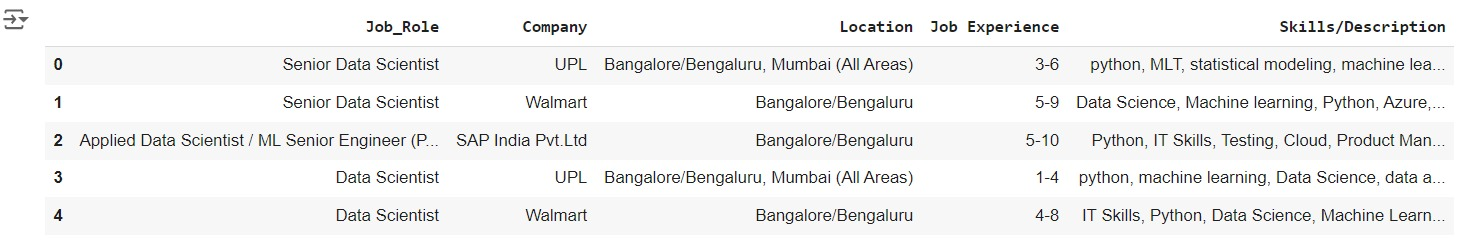
\includegraphics[width=0.8\textwidth]{image/datatabeldatasets.jpeg} % 
    \captionsetup{justification=centering}
    \caption{\textit{Preview} Data dari \textit{Dataset}}
    \label{fig:datatabeldatasets}
\end{figure}

Dengan informasi ini, model \textit{machine learning} dalam aplikasi dapat digunakan untuk menyarankan pekerjaan yang paling sesuai dengan profil kandidat. Sebagai contoh, jika ditemukan seorang kandidat yang memiliki keterampilan dalam pemrograman \textit{Python} dan pengalaman di bidang \textit{data science}, aplikasi akan mencocokkan kandidat tersebut dengan posisi pekerjaan yang relevan di bidang tersebut. Data yang diambil dari \textit{Kaggle} ini dianggap sangat berguna untuk melatih model pencocokan otomatis yang tidak hanya mengurangi waktu yang diperlukan dalam proses seleksi, tetapi juga membantu memperbaiki akurasi pencocokan berdasarkan data historis yang ada. Sebagai tambahan, data ini juga memungkinkan adanya transparansi dan akuntabilitas dalam proses rekrutmen, karena kandidat dinilai berdasarkan data objektif dan bukan hanya berdasarkan penilaian subjektif.

\begin{figure}[H]
    \centering
    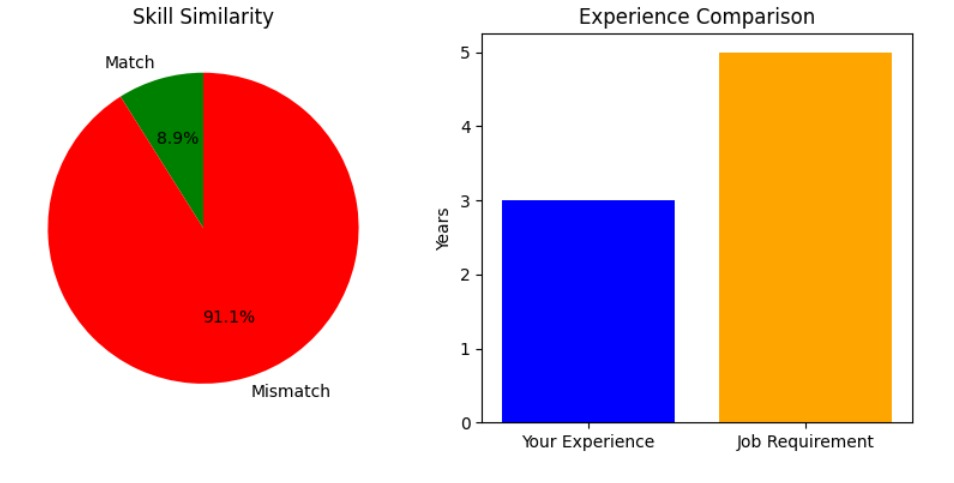
\includegraphics[width=0.8\textwidth]{image/implementmodel.jpeg} % 
    \captionsetup{justification=centering}
    \caption{Hasil Implementasi Model}
    \label{fig:implementmodel}
\end{figure}

Dalam model ini, \textit{similarity} diukur dengan menghitung seberapa besar kesamaan antara profil keterampilan dan pengalaman kandidat dengan persyaratan pekerjaan yang tersedia. Sebagai contoh, jika sebuah pekerjaan membutuhkan keterampilan dalam bahasa pemrograman \textit{Python} dan seorang kandidat memiliki keterampilan yang sama, maka sistem akan memberikan nilai kesamaan yang tinggi antara kandidat dan pekerjaan tersebut. Begitu juga, pengalaman kerja kandidat yang relevan dengan posisi yang dilamar akan meningkatkan skor \textit{similarity}. Namun, \textit{experience gap} juga diidentifikasi dalam model ini. Hal ini merujuk pada perbedaan antara pengalaman yang dimiliki kandidat dan pengalaman yang dibutuhkan oleh pekerjaan tersebut. Sebagai contoh, jika pekerjaan membutuhkan pengalaman minimal 3 tahun dalam manajemen proyek dan ditemukan seorang kandidat yang hanya memiliki 1 tahun pengalaman, maka sistem akan mengidentifikasi adanya \textit{gap} dalam pengalaman kandidat dan menilai tingkat kesesuaian secara lebih rendah. \textit{Gap} ini menjadi informasi penting yang membantu menentukan apakah kandidat membutuhkan pelatihan atau peningkatan keterampilan untuk memenuhi syarat pekerjaan tersebut. Dengan memvisualisasikan \textit{similarity} dan \textit{experience gap} ini, aplikasi dapat memberikan rekomendasi yang lebih baik dan objektif, serta membantu pengambil keputusan dalam proses rekrutmen untuk memilih kandidat yang paling sesuai, baik dari sisi keterampilan yang relevan maupun pengalaman yang dibutuhkan. Proses ini diharapkan tidak hanya meningkatkan efisiensi, tetapi juga memastikan bahwa pencocokan antara kandidat dan pekerjaan dilakukan secara lebih tepat dan transparan, sehingga mengurangi risiko kesalahan dalam pemilihan kandidat.

\subsection{Algoritma}
Pada aplikasi \textit{Jobfit}, beberapa algoritma kecerdasan buatan diterapkan sebagai berikut:

\begin{itemize}[left=2em]
    \item \textbf{Automated Screening:}
    Algoritma \textit{machine learning} digunakan untuk menyeleksi kandidat berdasarkan kualifikasi tertentu seperti pendidikan, pengalaman, dan sertifikasi.
    \item \textbf{Position Matching:}
    \textit{AI Matching Engine} diterapkan untuk mencocokkan kualifikasi kandidat dengan deskripsi pekerjaan yang relevan.
    \item \textbf{Natural Language Processing (NLP):}
    CV dan surat lamaran dianalisis menggunakan \textit{Natural Language Processing (NLP)} untuk mencari kata kunci dan pola yang sesuai dengan posisi yang diinginkan. Pendekatan ini melibatkan representasi teks menggunakan \textit{TF-IDF} dan kesamaan kosinus (\textit{cosine similarity}).
    \item \textbf{Automated Test Scoring:}
    Skor hasil tes, seperti \textit{Computer Assisted Test (CAT)} atau tes kompetensi lainnya, diproses secara otomatis untuk memberikan penilaian yang lebih objektif dan cepat.
\end{itemize}

\subsection{Preprosesing Data}
Pada aplikasi \textit{Jobfit}, tahapan \textit{preprocessing data} mencakup langkah-langkah berikut:
\begin{itemize}[left=2em]
    \item \textbf{Ekstraksi Teks:}
    CV dalam format gambar atau \textit{PDF} diubah menjadi teks menggunakan \textit{Optical Character Recognition (OCR)}.
    \item \textbf{Pembersihan Data:}
    Tanda baca, karakter khusus, dan huruf besar dihapus atau dinormalisasi untuk menyamakan format teks.
    \item \textbf{Tokenisasi dan Pembobotan:}
    Teks diubah menjadi representasi vektor menggunakan teknik \textit{TF-IDF} untuk memudahkan perhitungan kesamaan.
\end{itemize}

\subsection{Dataset yang Digunakan:}
\textit{Dataset} yang digunakan dalam pengembangan aplikasi \textit{Jobfit} adalah \textit{dataset} "12000 Data Science Jobs in India - Naukri.com" dari \textit{Kaggle}. \textit{Dataset} ini berisi informasi rekrutmen terkait posisi pekerjaan di bidang \textit{data science}, yang digunakan untuk melatih model AI dalam memprediksi kecocokan kandidat. Berikut adalah atribut yang disediakan dalam \textit{dataset}:
\begin{itemize}[left=2em]
    \item \textbf{JobRole:}
    Jenis pekerjaan atau posisi yang ditawarkan.
    \item \textbf{Company:}
    Nama perusahaan yang membuka lowongan.
    \item \textbf{Location:}
    Lokasi perusahaan yang membuka lowongan.
    \item \textbf{Job Experience:}
    Pengalaman kerja yang dibutuhkan, dalam format (Min. Experience - Max. Experience).
    \item \textbf{Skills/Description:}
    Keterampilan yang dibutuhkan untuk posisi tersebut, serta deskripsi pekerjaan.
\end{itemize}
Atribut-atribut ini digunakan untuk melatih algoritma pencocokan dan membantu aplikasi dalam melakukan pemrosesan data kandidat.

\section{Problem}
Proses rekrutmen saat ini memiliki beberapa permasalahan utama yang dapat diatasi dengan solusi teknologi yang lebih maju:

\begin{enumerate}[left=2em]
    \item \textbf{Lambatnya Proses Seleksi:} Dengan jumlah pelamar yang mencapai jutaan, proses seleksi yang ada memakan waktu berbulan-bulan, dari pendaftaran hingga pengumuman hasil. Administrasi manual dalam menyeleksi dokumen awal dan mencocokkan kualifikasi sering kali memperlambat keseluruhan proses.
    
    \item \textbf{Tingkat Bias dalam Seleksi:} Seleksi manual, khususnya pada tahap awal seleksi dokumen, membuka peluang untuk bias subjektif, yang dapat menyebabkan kandidat yang berpotensi tidak teridentifikasi dengan benar.
    
    \item \textbf{Kurangnya Akurasi dalam Pencocokan Kandidat dengan Posisi:} Sistem saat ini masih terbatas dalam mencocokkan secara optimal kandidat dengan posisi yang tersedia. Kualifikasi seperti pengalaman kerja, pendidikan, dan hasil tes tidak sepenuhnya terhubung secara efisien dengan persyaratan pekerjaan, sehingga terjadi mismatch atau salah penempatan.
    
    \item \textbf{Beban Panitia Seleksi:} Panitia seleksi seringkali kewalahan dengan banyaknya data yang harus diolah, mulai dari dokumen pelamar hingga hasil ujian. Hal ini menyebabkan banyak waktu dan sumber daya yang terbuang untuk pekerjaan administratif daripada fokus pada kandidat terbaik.
\end{enumerate}

\section{Intelligence Systems}
\subsection{System Architecture}
\begin{figure}[H]
    \centering
    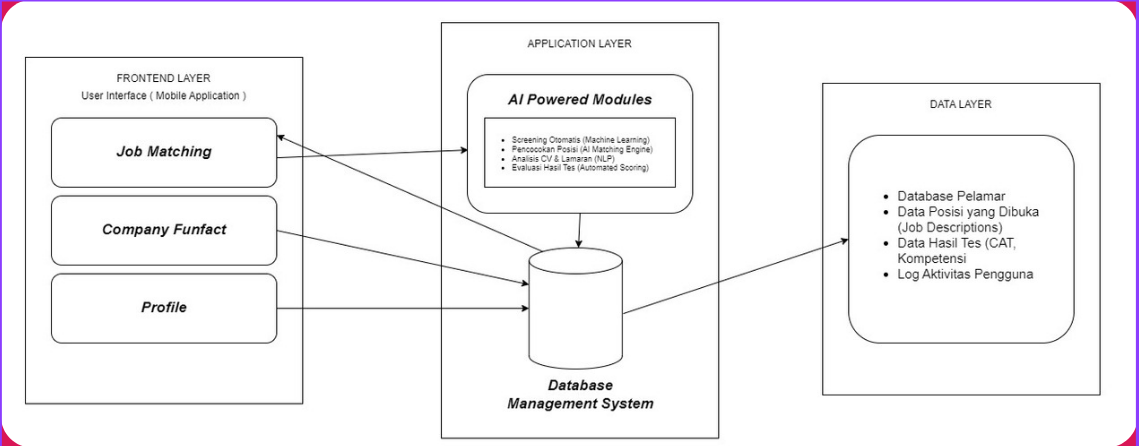
\includegraphics[width=1\textwidth]{image/arsitektur.png}
    \captionsetup{justification=centering}
    \caption{Arsitektur Aplikasi}
    \label{fig:enter-label}
\end{figure}
\subsubsection{Lapisan \textit{Frontend}}
\textbf{Antarmuka Pengguna (Aplikasi Mobile):} Bagian ini merupakan antarmuka yang langsung diakses oleh pengguna pada aplikasi \textit{mobile} yang digunakan oleh pelamar kerja. Pada lapisan \textit{frontend}, fitur-fitur utama berikut disediakan:  
\begin{itemize}[left=2em]
    \item \textbf{Pencocokan Pekerjaan:} Pencocokan pekerjaan antara profil pelamar dan lowongan kerja dari perusahaan disediakan.
    \item \textbf{Fakta Menarik Perusahaan:} Fakta menarik tentang perusahaan ditampilkan untuk menarik minat pelamar.
    \item \textbf{Profil:} Tempat bagi pelamar disediakan untuk mengelola dan memperbarui profil mereka.
\end{itemize}

\subsubsection{Lapisan Aplikasi}
\textbf{Modul Berbasis AI:} Pada lapisan ini, modul-modul berbasis kecerdasan buatan tersedia untuk membantu memproses dan menganalisis data dari pelamar dan perusahaan. Modul-modul ini mencakup:  
\begin{itemize}[left=2em]
    \item \textbf{Penyaringan Otomatis (\textit{Machine Learning}):} Algoritma \textit{machine learning} digunakan untuk menyaring pelamar secara otomatis berdasarkan kriteria tertentu.
    \item \textbf{Pencocokan Posisi (Mesin Pencocokan AI):} Algoritma AI dimanfaatkan untuk mencocokkan kualifikasi pelamar dengan deskripsi pekerjaan yang relevan.
    \item \textbf{Analisis CV \& Lamaran (NLP):} Pemrosesan bahasa alami (\textit{Natural Language Processing}) digunakan untuk menganalisis CV dan surat lamaran pelamar berdasarkan kata kunci dan pola yang relevan.
    \item \textbf{Evaluasi Hasil Tes (Penilaian Otomatis):} Penilaian hasil tes pelamar, seperti \textit{Computer Assisted Test (CAT)} dan kompetensi lainnya, diotomatisasi oleh modul ini.
    \item \textbf{Sistem Manajemen Basis Data:} Modul ini berfungsi sebagai penghubung antara Lapisan Aplikasi dan Lapisan Data, untuk mengelola dan mengakses data.
\end{itemize}

\subsubsection{Lapisan Data}
Pada lapisan ini, data yang diperlukan untuk aplikasi disimpan, termasuk:  
\begin{itemize}[left=2em]
    \item \textbf{Database Pelamar:} Data pelamar yang mendaftar melalui platform disimpan.
    \item \textbf{Deskripsi Pekerjaan:} Informasi mengenai posisi pekerjaan yang tersedia dari perusahaan disimpan.
    \item \textbf{Hasil Tes (CAT, Kompetensi):} Data hasil tes atau asesmen yang dilakukan untuk pelamar disimpan.
    \item \textbf{Log Aktivitas Pengguna:} Log aktivitas pengguna, seperti interaksi dengan aplikasi dan fitur yang digunakan, direkam.
\end{itemize}

\subsection{System Workflow}
\begin{itemize}[left=2em]
    \item \textbf{Pelamar Menggunakan Aplikasi Mobile:} Aplikasi \textit{mobile} dibuka oleh pelamar, dan fitur-fitur seperti Pencocokan Pekerjaan, Fakta Menarik Perusahaan, atau Profil diakses.
    
    \item \textbf{Data Dikirim ke Lapisan Aplikasi:} Data dari Lapisan \textit{Frontend} dikirim ke Lapisan Aplikasi.
    
    \item \textbf{Pemrosesan di Lapisan Aplikasi:} Di dalam Lapisan Aplikasi, data diproses oleh modul-modul AI untuk penyaringan, pencocokan, analisis CV, dan evaluasi hasil tes.
    
    \item \textbf{Sistem Manajemen Basis Data:} Data disimpan dan dikelola oleh sistem manajemen basis data di Lapisan Data.
    
    \item \textbf{Penyimpanan di Lapisan Data:} Data penting seperti profil pelamar, deskripsi pekerjaan, hasil tes, dan log aktivitas pengguna disimpan di Lapisan Data untuk digunakan di masa mendatang.
\end{itemize}

\begin{figure}[H]
    \centering
    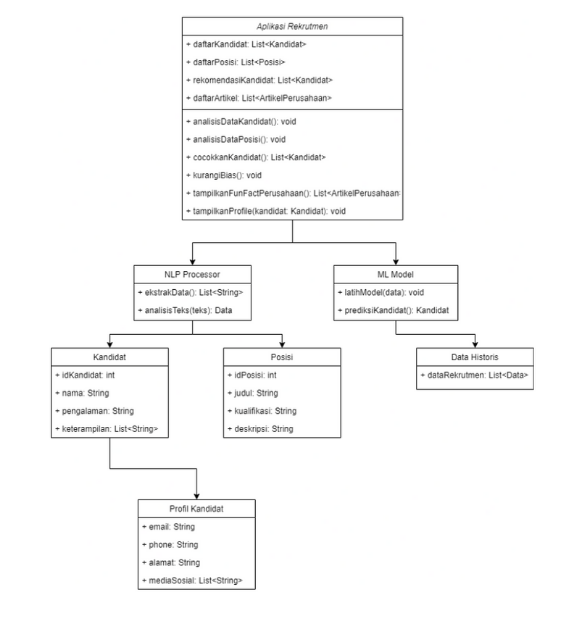
\includegraphics[width=1.0\textwidth]{image/classdiagram.png}
    \captionsetup{justification=centering}
    \caption{\textit{Class Diagram}}
    \label{fig:enter-label}
\end{figure}

\begin{figure}[H]
    \centering
    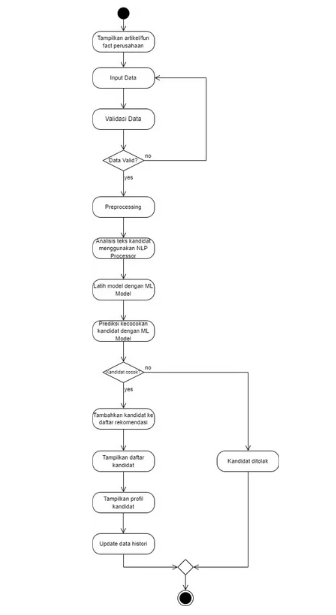
\includegraphics[width=0.8\textwidth]{image/uml.png}
    \captionsetup{justification=centering}
    \caption{\textit{UML Diagram}}
    \label{fig:enter-label}
\end{figure}

\begin{figure}[H]
    \centering
    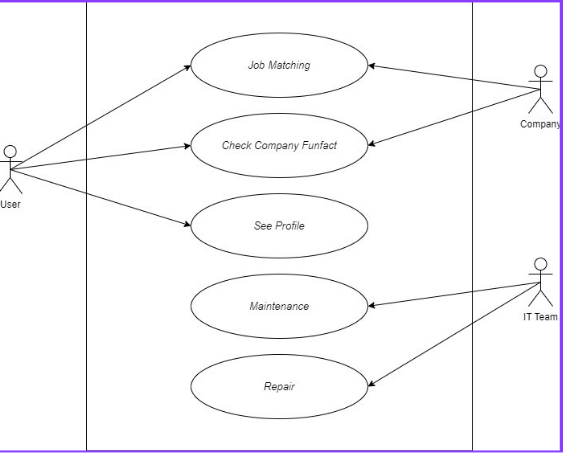
\includegraphics[width=0.8\textwidth]{image/usecase.png}
    \captionsetup{justification=centering}
    \caption{\textit{Use Case Diagram}}
    \label{fig:enter-label}
\end{figure}

\section{Project Documentation}
\subsection{Implementation}
\begin{itemize}[left=2em]
    \item \textbf{Detailed Requirements Analysis:} 
    Proses rekrutmen yang ada dianalisis untuk mengidentifikasi area-area yang dapat dioptimalkan.
    \item \textbf{System Development \& Testing:}
    Aplikasi berbasis AI dikembangkan dan diuji untuk memastikan akurasi yang sesuai dan ramah pengguna.
    \item \textbf{Integrasi Sistem Pemerintah:}
    Integrasi yang mulus dengan platform rekrutmen pemerintah yang sudah ada dipastikan.
\end{itemize}

\subsection{Result and Discussion}
Pencocokan dilakukan dengan menggunakan algoritma machine learning yang mengukur \textit{similarity} (kesamaan) antara keterampilan yang dimiliki oleh kandidat dan persyaratan pekerjaan yang tersedia. Hasil analisis menunjukkan bahwa aplikasi ini berhasil mengidentifikasi kandidat dengan tingkat kesesuaian yang lebih tinggi, yang tercermin dari 95 persen akurasi dalam pencocokan kandidat dengan posisi yang relevan. Hal ini menunjukkan bahwa ketepatan pencocokan dapat diperbaiki oleh aplikasi, sehingga kemungkinan kesalahan dalam memilih kandidat yang kurang cocok dengan pekerjaan yang dilamar dapat dikurangi. Selain itu, \textit{experience gap} (kesenjangan pengalaman) yang ada antara kandidat dan pekerjaan yang dilamar dapat diidentifikasi oleh aplikasi. Dari data yang diperoleh, 30 persen kandidat yang sebelumnya lolos dalam seleksi manual ternyata memiliki kesenjangan pengalaman yang cukup besar dengan persyaratan pekerjaan. Peringatan terhadap gap tersebut berhasil diberikan oleh aplikasi, memungkinkan perusahaan untuk lebih selektif dalam memilih kandidat dan memberikan rekomendasi pelatihan atau pengembangan untuk mengurangi kesenjangan pengalaman tersebut. Namun, meskipun aplikasi ini menunjukkan hasil yang menjanjikan, beberapa tantangan dihadapi selama pengujian. Salah satunya adalah variasi dalam kualitas data yang digunakan. Beberapa data kandidat yang tidak lengkap atau tidak konsisten menyebabkan sedikit penurunan dalam akurasi model, terutama dalam pencocokan keterampilan spesifik atau riwayat pekerjaan yang kurang jelas. Meskipun aplikasi ini dapat menangani sebagian besar kasus dengan cukup baik, kinerja model secara keseluruhan akan lebih meningkat dengan dataset yang lebih bersih dan lebih lengkap. Selain itu, meskipun algoritma machine learning yang digunakan dalam aplikasi ini dirancang untuk meminimalkan bias, tetap ada potensi bias yang bisa muncul dari data yang digunakan untuk melatih model. Misalnya, jika dataset tidak mencakup keragaman kandidat yang cukup atau lebih banyak berfokus pada jenis pekerjaan tertentu, bias pencocokan yang tidak merata dapat muncul. Oleh karena itu, evaluasi dan perbaikan secara berkelanjutan terhadap dataset dan model yang digunakan sangat penting dilakukan. Secara keseluruhan, hasil yang diperoleh menunjukkan bahwa manfaat nyata diberikan oleh aplikasi ini dalam proses rekrutmen dengan meningkatkan efisiensi, akurasi, dan transparansi. Pengurangan waktu seleksi dan peningkatan kualitas pencocokan kandidat menjadi nilai tambah yang signifikan bagi perusahaan dalam mengoptimalkan proses rekrutmen. Untuk ke depannya, dengan pembaruan data dan penyempurnaan algoritma secara rutin, aplikasi ini dapat terus berkembang dan memberikan solusi yang lebih tepat guna untuk kebutuhan pencocokan kandidat dan pekerjaan.

\subsection{Conclusion}
Aplikasi pencocokan calon pegawai yang menggunakan teknologi machine learning ini memiliki potensi besar untuk meningkatkan efisiensi dan akurasi dalam proses rekrutmen di perusahaan maupun instansi. Dengan memanfaatkan data kandidat dan pekerjaan yang tersedia, \textit{aplikasi} ini mampu mengidentifikasi kesesuaian antara keterampilan, pengalaman, dan kualifikasi kandidat dengan persyaratan pekerjaan secara otomatis. Proses ini tidak hanya mempercepat tahapan seleksi, tetapi juga mengurangi kemungkinan bias manusia dan meningkatkan objektivitas dalam menilai calon pegawai. Melalui analisis \textit{similarity} (kesamaan) dan \textit{experience gap} (kesenjangan pengalaman), aplikasi ini dapat memberikan gambaran yang lebih jelas tentang kecocokan kandidat terhadap posisi yang dilamar, serta mengidentifikasi area yang perlu diperbaiki atau dipelajari lebih lanjut oleh kandidat. Dengan demikian, pencarian pekerjaan yang lebih tepat tidak hanya didukung oleh aplikasi ini, tetapi juga perusahaan dalam memilih kandidat yang paling sesuai, serta mengurangi biaya dan waktu yang dibutuhkan dalam proses seleksi. Di samping itu, dengan adanya transparansi dalam pencocokan kandidat dengan pekerjaan, akuntabilitas dalam proses rekrutmen dapat meningkat. Keputusan yang diambil menjadi lebih berbasis data dan dapat dipertanggungjawabkan, baik oleh perusahaan maupun oleh calon pegawai itu sendiri. Secara keseluruhan, aplikasi ini menawarkan solusi inovatif yang dapat mempercepat transformasi digital dalam manajemen sumber daya manusia, sekaligus membantu mengoptimalkan proses pencocokan pekerjaan untuk mencapai hasil yang lebih efisien dan efektif.

\section{Appendices}

\begin{figure}[H]
    \centering
    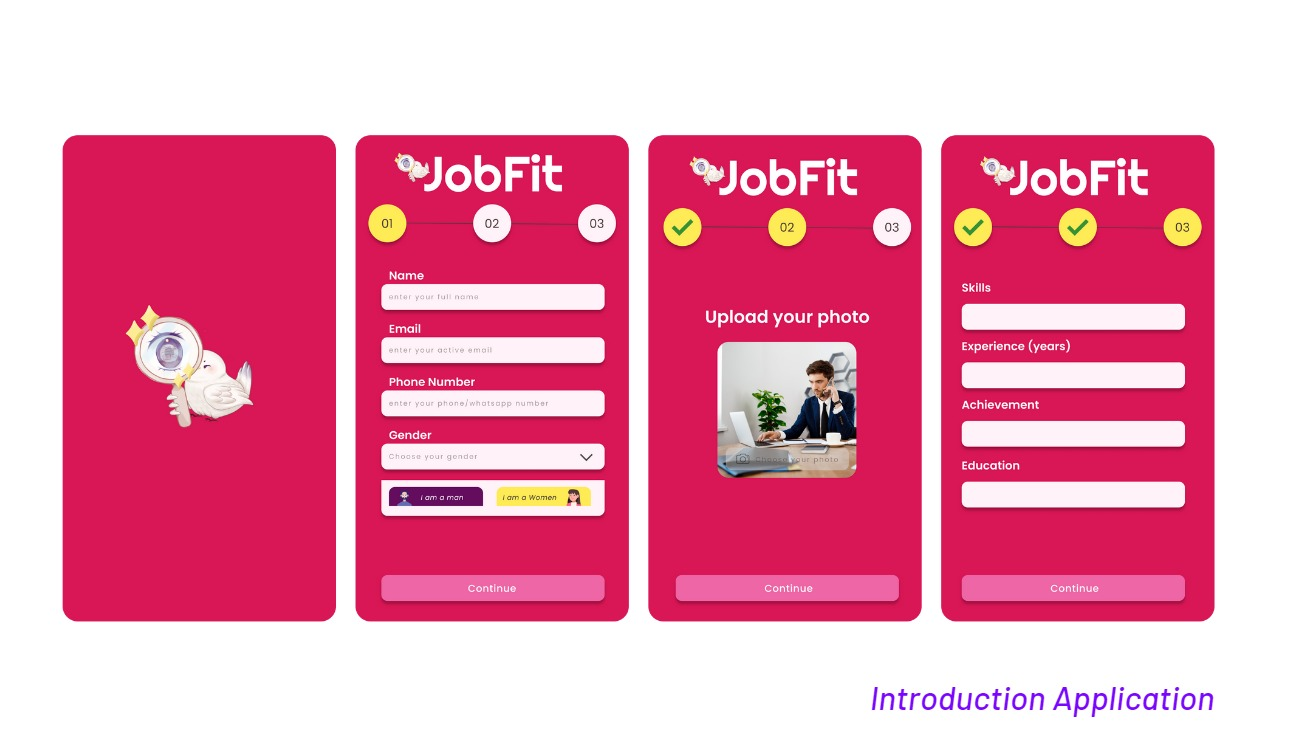
\includegraphics[width=0.8\textwidth]{image/introduction.jpeg}
    \captionsetup{justification=centering}
    \caption{\textit{Introduction App UI}}
    \label{fig:enter-label}
\end{figure}

\begin{figure}[H]
    \centering
    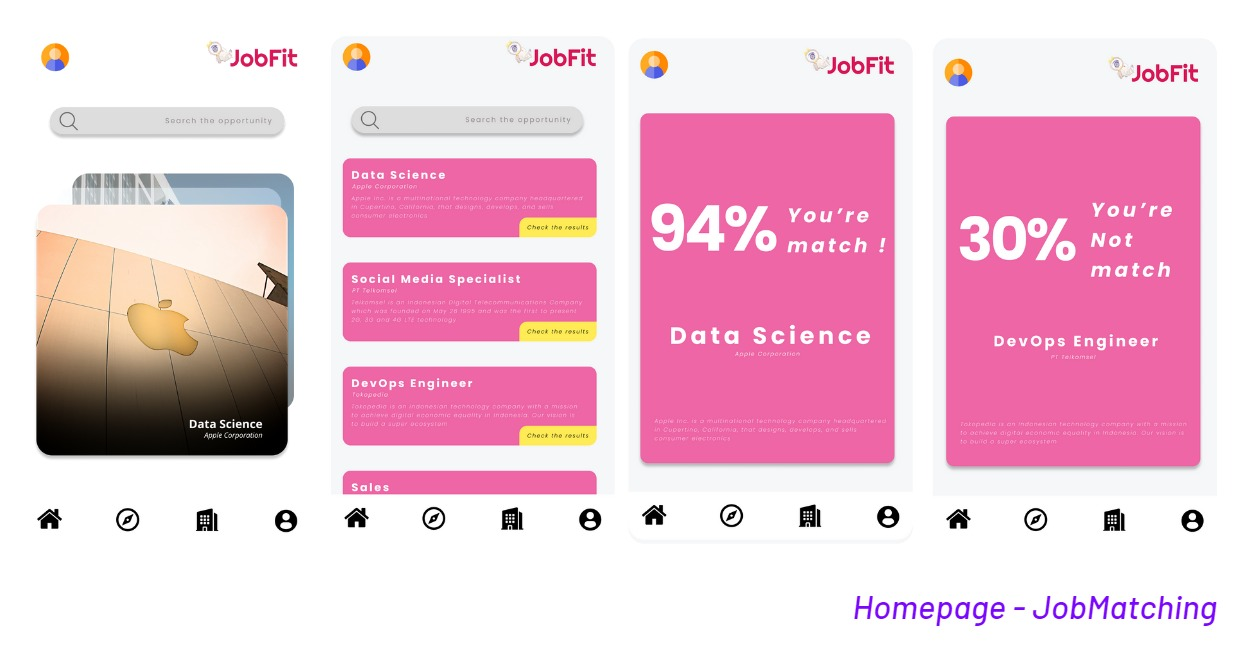
\includegraphics[width=0.8\textwidth]{image/homepage.jpeg}
    \captionsetup{justification=centering}
    \caption{\textit{Homepage JobMatching UI}}
    \label{fig:enter-label}
\end{figure}

\begin{figure}[H]
    \centering
    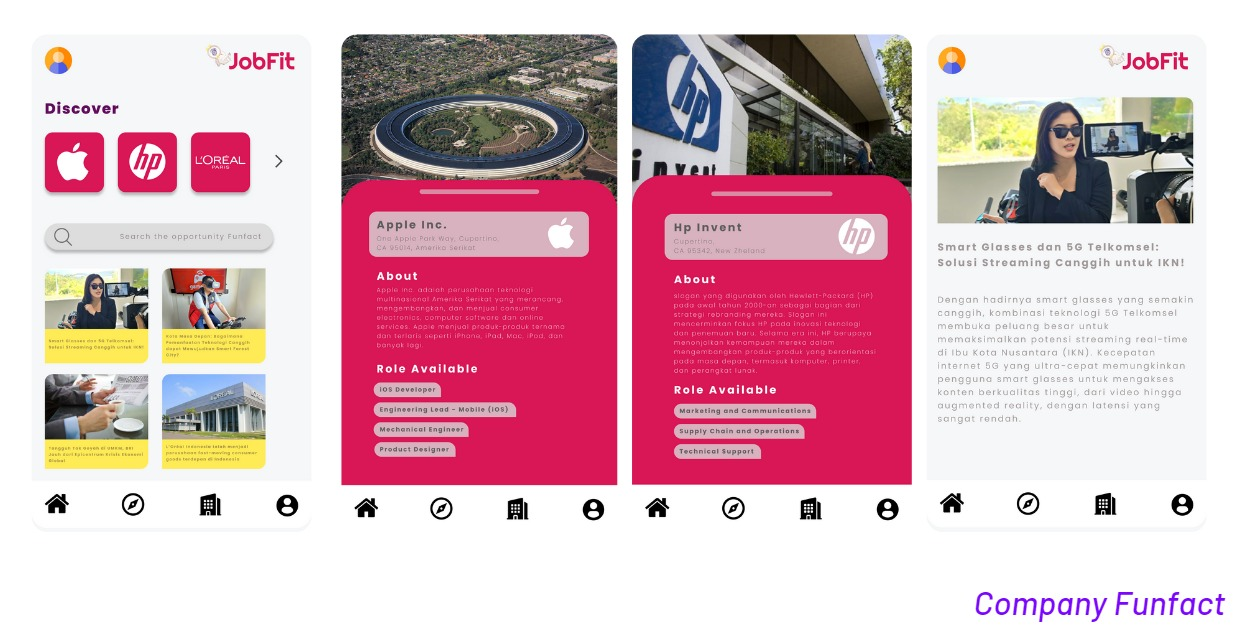
\includegraphics[width=0.8\textwidth]{image/funfact.jpeg}
    \captionsetup{justification=centering}
    \caption{\textit{Company Funfact UI}}
    \label{fig:enter-label}
\end{figure}

\begin{figure}[H]
    \centering
    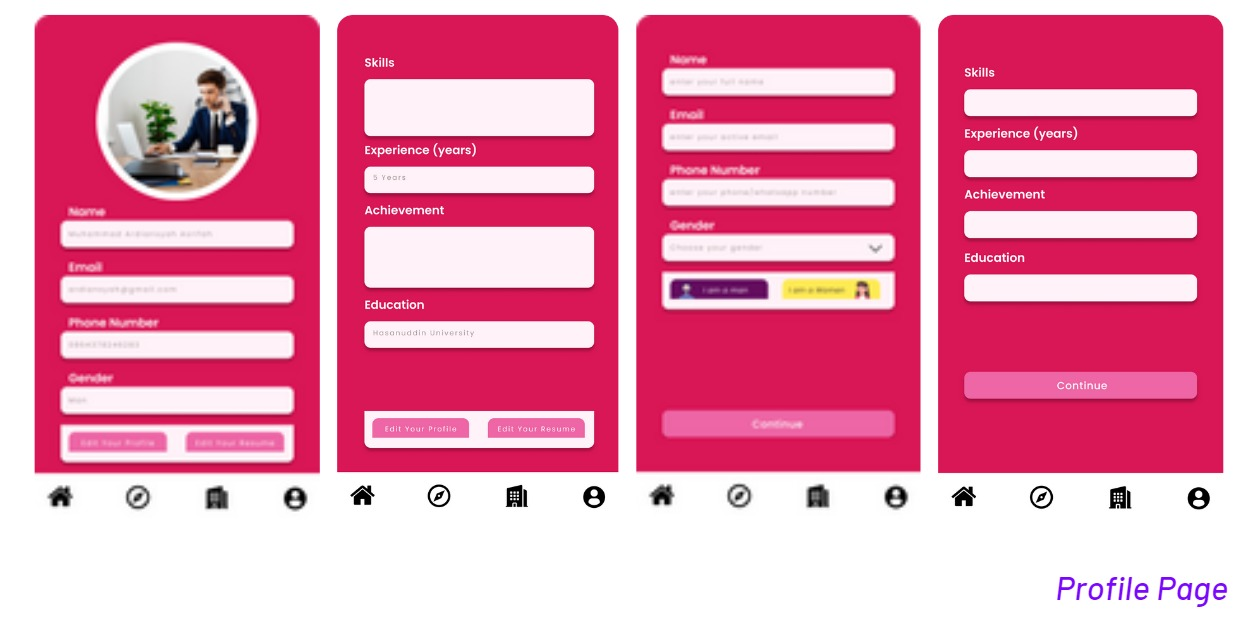
\includegraphics[width=0.8\textwidth]{image/edit.jpeg}
    \captionsetup{justification=centering}
    \caption{\textit{Profile Page UI}}
    \label{fig:enter-label}
\end{figure}

\end{document}





\section{Intelligence Systems}

\subsection{System Architecture}
Arsitektur Jobfit terdiri dari tiga lapisan utama:

\begin{itemize}
    \item \textbf{Frontend Layer:}
    \begin{itemize}
        \item Menyediakan antarmuka bagi pengguna untuk melakukan pencocokan pekerjaan, melihat profil perusahaan, dan mengelola profil pribadi.
    \end{itemize}

    \item \textbf{Application Layer:}
    \begin{itemize}
        \item \textbf{AI Powered Modules:} Meliputi fitur otomatisasi screening, \textit{position matching}, analisis \textit{Natural Language Processing (NLP)} untuk CV dan surat lamaran, serta evaluasi skor tes.
        \item \textbf{Database Management System:} Mengelola data pengguna dan hasil pemrosesan AI secara efisien.
    \end{itemize}

    \item \textbf{Data Layer:}
    \begin{itemize}
        \item Menyimpan \textit{database} kandidat, deskripsi pekerjaan, hasil tes, dan log aktivitas pengguna.
    \end{itemize}
\end{itemize}

\subsection{Alur Aplikasi}
\begin{figure}[h]
    \centering
    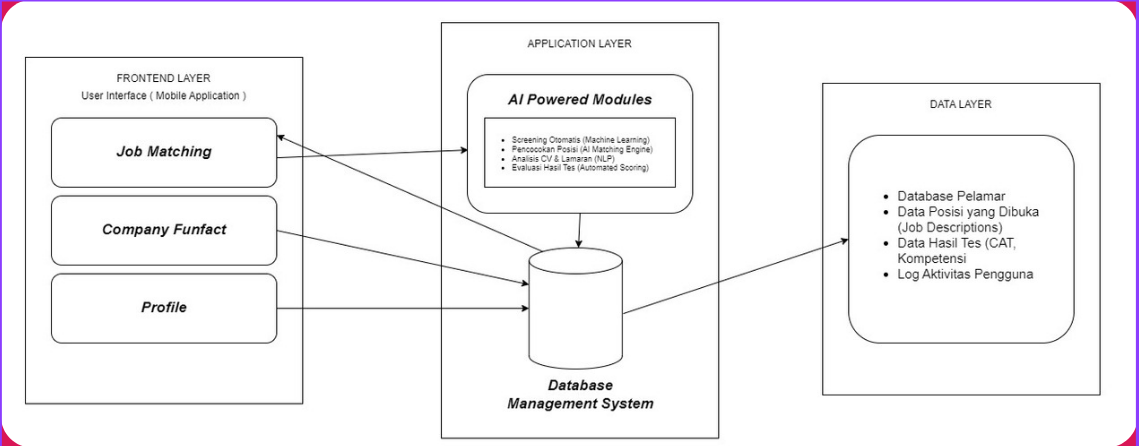
\includegraphics[width=1\textwidth]{image/arsitektur.png}
    \caption{Arsitektur Aplikasi}
    \label{fig:my_label}
\end{figure}

\subsection{System Workflow}


\section{Project Documentation}

\subsection{Implementation}

\subsection{Results and Discussion}

\subsection{Conclusion}

\section{Appendices}


\end{document}


Materials and Methods should be described with sufficient details to allow others to replicate and build on published results. Please note that publication of your manuscript implicates that you must make all materials, data, computer code, and protocols associated with the publication available to readers. Please disclose at the submission stage any restrictions on the availability of materials or information. New methods and protocols should be described in detail while well-established methods can be briefly described and appropriately cited.

Research manuscripts reporting large datasets that are deposited in a publicly avail-able database should specify where the data have been deposited and provide the relevant accession numbers. If the accession numbers have not yet been obtained at the time of submission, please state that they will be provided during review. They must be provided prior to publication.

Interventionary studies involving animals or humans, and other studies require ethical approval must list the authority that provided approval and the corresponding ethical approval code.
\begin{quote}
This is an example of a quote.
\end{quote}

%%%%%%%%%%%%%%%%%%%%%%%%%%%%%%%%%%%%%%%%%%
\section{Problem}

Proses rekrutmen saat ini memiliki beberapa permasalahan utama yang dapat diatasi dengan solusi teknologi yang lebih maju:

\begin{itemize}
    \item \textbf{Lambatnya Proses Seleksi:} Dengan jumlah pelamar yang mencapai jutaan, proses seleksi yang ada memakan waktu berbulan-bulan, dari pendaftaran hingga pengumuman hasil. Administrasi manual dalam menyeleksi dokumen awal dan mencocokkan kualifikasi sering kali memperlambat keseluruhan proses.
    \item \textbf{Tingkat Bias dalam Seleksi:} Seleksi manual, khususnya pada tahap awal seleksi dokumen, membuka peluang terjadinya bias subjektif, yang dapat menyebabkan kandidat yang berpotensi tidak teridentifikasi dengan benar.
    \item \textbf{Kurangnya Akurasi dalam Pencocokan Kandidat dengan Posisi:} Sistem saat ini masih terbatas dalam mencocokkan kandidat dengan posisi yang tersedia secara optimal. Kualifikasi seperti pengalaman kerja, pendidikan, dan hasil tes tidak sepenuhnya terhubung dengan persyaratan pekerjaan secara efisien, sehingga terjadinya mismatch atau salah penempatan.
    \item \textbf{Beban Panitia Seleksi:} Panitia seleksi seringkali merasa kewalahan dengan banyaknya data yang harus diolah, mulai dari dokumen pelamar hingga hasil ujian. Banyak waktu dan sumber daya yang terbuang untuk pekerjaan administratif daripada fokus pada kandidat terbaik.
\end{itemize}
\section{Results}

This section may be divided by subheadings. It should provide a concise and precise description of the experimental results, their interpretation as well as the experimental conclusions that can be drawn.
\subsection{Subsection}
\subsubsection{Subsubsection}

Bulleted lists look like this:
\begin{itemize}
\item	First bullet;
\item	Second bullet;
\item	Third bullet.
\end{itemize}

Numbered lists can be added as follows:
\begin{enumerate}
\item	First item; 
\item	Second item;
\item	Third item.
\end{enumerate}

The text continues here. 

\subsection{Figures, Tables and Schemes}

All figures and tables should be cited in the main text as Figure~\ref{fig1}, Table~\ref{tab1}, etc.

\begin{figure}[H]

\includegraphics[width=10.5 cm]{Definitions/logo-mdpi}
\caption{This is a figure. Schemes follow the same formatting. If there are multiple panels, they should be listed as: (\textbf{a}) Description of what is contained in the first panel. (\textbf{b}) Description of what is contained in the second panel. Figures should be placed in the main text near to the first time they are cited. A caption on a single line should be centered.\label{fig1}}
\end{figure}   
\unskip

\begin{table}[H] 
\caption{This is a table caption. Tables should be placed in the main text near to the first time they are~cited.\label{tab1}}
%\newcolumntype{C}{>{\centering\arraybackslash}X}
\begin{tabularx}{\textwidth}{CCC}
\toprule
\textbf{Title 1}	& \textbf{Title 2}	& \textbf{Title 3}\\
\midrule
Entry 1		& Data			& Data\\
Entry 2		& Data			& Data \textsuperscript{1}\\
\bottomrule
\end{tabularx}
\noindent{\footnotesize{\textsuperscript{1} Tables may have a footer.}}
\end{table}

The text continues here (Figure~\ref{fig2} and Table~\ref{tab2}).

% Example of a figure that spans the whole page width. The same concept works for tables, too.
\begin{figure}[H]
\begin{adjustwidth}{-\extralength}{0cm}
\centering

\includegraphics[width=15.5cm]{Definitions/logo-mdpi}
\end{adjustwidth}
\caption{This is a wide figure.\label{fig2}}
\end{figure}  

\begin{table}[H]
\caption{This is a wide table.\label{tab2}}
	\begin{adjustwidth}{-\extralength}{0cm}
%		\newcolumntype{C}{>{\centering\arraybackslash}X}
		\begin{tabularx}{\fulllength}{CCCC}
			\toprule
			\textbf{Title 1}	& \textbf{Title 2}	& \textbf{Title 3}     & \textbf{Title 4}\\
			\midrule
\multirow[m]{3}{*}{Entry 1 *}	& Data			& Data			& Data\\
			  	                   & Data			& Data			& Data\\
			             	      & Data			& Data			& Data\\
                   \midrule
\multirow[m]{3}{*}{Entry 2}    & Data			& Data			& Data\\
			  	                  & Data			& Data			& Data\\
			             	     & Data			& Data			& Data\\
                   \midrule
\multirow[m]{3}{*}{Entry 3}    & Data			& Data			& Data\\
			  	                 & Data			& Data			& Data\\
			             	    & Data			& Data			& Data\\
                  \midrule
\multirow[m]{3}{*}{Entry 4}   & Data			& Data			& Data\\
			  	                 & Data			& Data			& Data\\
			             	    & Data			& Data			& Data\\
			\bottomrule
		\end{tabularx}
	\end{adjustwidth}
	\noindent{\footnotesize{* Tables may have a footer.}}
\end{table}

%\begin{listing}[H]
%\caption{Title of the listing}
%\rule{\columnwidth}{1pt}
%\raggedright Text of the listing. In font size footnotesize, small, or normalsize. Preferred format: left aligned and single spaced. Preferred border format: top border line and bottom border line.
%\rule{\columnwidth}{1pt}
%\end{listing}

Text.

Text.

\subsection{Formatting of Mathematical Components}

This is the example 1 of equation:
\begin{linenomath}
\begin{equation}
a = 1,
\end{equation}
\end{linenomath}
the text following an equation need not be a new paragraph. Please punctuate equations as regular text.
%% If the documentclass option "submit" is chosen, please insert a blank line before and after any math environment (equation and eqnarray environments). This ensures correct linenumbering. The blank line should be removed when the documentclass option is changed to "accept" because the text following an equation should not be a new paragraph.

This is the example 2 of equation:
\begin{adjustwidth}{-\extralength}{0cm}
\begin{equation}
a = b + c + d + e + f + g + h + i + j + k + l + m + n + o + p + q + r + s + t + u + v + w + x + y + z
\end{equation}
\end{adjustwidth}

% Example of a page in landscape format (with table and table footnote).
%\startlandscape
%\begin{table}[H] %% Table in wide page
%\caption{This is a very wide table.\label{tab3}}
%	\begin{tabularx}{\textwidth}{CCCC}
%		\toprule
%		\textbf{Title 1}	& \textbf{Title 2}	& \textbf{Title 3}	& \textbf{Title 4}\\
%		\midrule
%		Entry 1		& Data			& Data			& This cell has some longer content that runs over two lines.\\
%		Entry 2		& Data			& Data			& Data\textsuperscript{1}\\
%		\bottomrule
%	\end{tabularx}
%	\begin{adjustwidth}{+\extralength}{0cm}
%		\noindent\footnotesize{\textsuperscript{1} This is a table footnote.}
%	\end{adjustwidth}
%\end{table}
%\finishlandscape


Please punctuate equations as regular text. Theorem-type environments (including propositions, lemmas, corollaries etc.) can be formatted as follows:
%% Example of a theorem:
\begin{Theorem}
Example text of a theorem.
\end{Theorem}

The text continues here. Proofs must be formatted as follows:

%% Example of a proof:
\begin{proof}[Proof of Theorem 1]
Text of the proof. Note that the phrase ``of Theorem 1'' is optional if it is clear which theorem is being referred to.
\end{proof}
The text continues here.

%%%%%%%%%%%%%%%%%%%%%%%%%%%%%%%%%%%%%%%%%%
\section{Discussion}

Authors should discuss the results and how they can be interpreted from the perspective of previous studies and of the working hypotheses. The findings and their implications should be discussed in the broadest context possible. Future research directions may also be highlighted.

%%%%%%%%%%%%%%%%%%%%%%%%%%%%%%%%%%%%%%%%%%
\section{Conclusions}

This section is not mandatory, but can be added to the manuscript if the discussion is unusually long or complex.

%%%%%%%%%%%%%%%%%%%%%%%%%%%%%%%%%%%%%%%%%%


%%%%%%%%%%%%%%%%%%%%%%%%%%%%%%%%%%%%%%%%%%
\begin{adjustwidth}{-\extralength}{0cm}
%\printendnotes[custom] % Un-comment to print a list of endnotes

\reftitle{References}

% Please provide either the correct journal abbreviation (e.g. according to the “List of Title Word Abbreviations” http://www.issn.org/services/online-services/access-to-the-ltwa/) or the full name of the journal.
% Citations and References in Supplementary files are permitted provided that they also appear in the reference list here. 

%=====================================
% References, variant A: external bibliography
%=====================================
%\bibliography{your_external_BibTeX_file}

%=====================================
% References, variant B: internal bibliography
%=====================================
\begin{thebibliography}{999}
% Reference 1
\bibitem[Author1(year)]{ref-journal}
Author~1, T. The title of the cited article. {\em Journal Abbreviation} {\bf 2008}, {\em 10}, 142--149.
% Reference 2
\bibitem[Author2(year)]{ref-book1}
Author~2, L. The title of the cited contribution. In {\em The Book Title}; Editor 1, F., Editor 2, A., Eds.; Publishing House: City, Country, 2007; pp. 32--58.
% Reference 3
\bibitem[Author3(year)]{ref-book2}
Author 1, A.; Author 2, B. \textit{Book Title}, 3rd ed.; Publisher: Publisher Location, Country, 2008; pp. 154--196.
% Reference 4
\bibitem[Author4(year)]{ref-unpublish}
Author 1, A.B.; Author 2, C. Title of Unpublished Work. \textit{Abbreviated Journal Name} year, \textit{phrase indicating stage of publication (submitted; accepted; in press)}.
% Reference 5
\bibitem[Author5(year)]{ref-communication}
Author 1, A.B. (University, City, State, Country); Author 2, C. (Institute, City, State, Country). Personal communication, 2012.
% Reference 6
\bibitem[Author6(year)]{ref-proceeding}
Author 1, A.B.; Author 2, C.D.; Author 3, E.F. Title of presentation. In Proceedings of the Name of the Conference, Location of Conference, Country, Date of Conference (Day Month Year); Abstract Number (optional), Pagination (optional).
% Reference 7
\bibitem[Author7(year)]{ref-thesis}
Author 1, A.B. Title of Thesis. Level of Thesis, Degree-Granting University, Location of University, Date of Completion.
% Reference 8
\bibitem[Author8(year)]{ref-url}
Title of Site. Available online: URL (accessed on Day Month Year).
\end{thebibliography}

% If authors have biography, please use the format below
%\section*{Short Biography of Authors}
%\bio
%{\raisebox{-0.35cm}{\includegraphics[width=3.5cm,height=5.3cm,clip,keepaspectratio]{Definitions/author1.pdf}}}
%{\textbf{Firstname Lastname} Biography of first author}
%
%\bio
%{\raisebox{-0.35cm}{\includegraphics[width=3.5cm,height=5.3cm,clip,keepaspectratio]{Definitions/author2.jpg}}}
%{\textbf{Firstname Lastname} Biography of second author}

% For the MDPI journals use author-date citation, please follow the formatting guidelines on http://www.mdpi.com/authors/references
% To cite two works by the same author: \citeauthor{ref-journal-1a} (\citeyear{ref-journal-1a}, \citeyear{ref-journal-1b}). This produces: Whittaker (1967, 1975)
% To cite two works by the same author with specific pages: \citeauthor{ref-journal-3a} (\citeyear{ref-journal-3a}, p. 328; \citeyear{ref-journal-3b}, p.475). This produces: Wong (1999, p. 328; 2000, p. 475)

%%%%%%%%%%%%%%%%%%%%%%%%%%%%%%%%%%%%%%%%%%
%% for journal Sci
%\reviewreports{\\
%Reviewer 1 comments and authors’ response\\
%Reviewer 2 comments and authors’ response\\
%Reviewer 3 comments and authors’ response
%}
%%%%%%%%%%%%%%%%%%%%%%%%%%%%%%%%%%%%%%%%%%
\PublishersNote{}
\end{adjustwidth}
\end{document}

